\begin{enumerate}[label=\thesubsection.\arabic*.,ref=\thesubsection.\theenumi]
\numberwithin{equation}{enumi}

\item The impulse response of a system is h\brak{t}= tu\brak{t}. For an input u\brak{t-1}, the output is:\\

\solution The Impulse response of the system is given by:
\begin{align}h\brak{t}= tu\brak{t}
\end{align}
Input:
\begin{align}x\brak{t}=u\brak{t-1}
\end{align}
The output will be given by:
\begin{align}y\brak{t}= x\brak{t}\ast h\brak{t}
\end{align}

%
\item We find the output using Laplace Transformation.
\\
In Laplace domain Convolution becomes Multiplication.
\begin{align}
F\brak{y\brak{t}}=F{x\brak{t}} F{h\brak{t}}
\\
\implies Y\brak{s}=\frac{e^{-s}}{s} \frac{1}{s^{2}}
\\
\implies Y\brak{s}=\frac{e^{-s}}{s^{3}}
\end{align}
\item Since we want the output in time domain we find the inverse Laplace Transform using Contour Integration.\\
The Inverse Laplace Transform :
\begin{align}
y\brak{t} = \frac{1}{2i\pi}\oint_C Y\brak{s}e^{st} \,ds\\
\implies y\brak{t}=\frac{1}{2i\pi}2i\pi\sum Res Y\brak{s}e^{st}
\end{align}
\\
\item Calculating the Residue.
\\
\begin{align}
Res_{s=s_o}=\frac{1}{\brak{p-1}!} \lim_{s\to s_{o}}  \frac{d^{p-1} }{d x^{p-1}}\sbrak{\brak{s-s_{o}}^p f\brak{s}}
\end{align}
where p denotes the number of times the pole is repeated.\\
\begin{align}
ResY\brak{s}e^{st}=\frac{1}{(3-1)!}\lim_{s\to 0}  \frac{d^{3-1}}{d x^{3-1}} \brak{s-0}^{3}
\frac{e^{s\brak{t-1}}}{s^{3}}\\
\implies ResY\brak{s}e^{st} = \frac{1}{2!}\lim_{s\to 0}  \frac{d^{2} }{d x^{2}} 
{e^{s\brak{t-1}}}\\
\implies ResY\brak{s}e^{st} = \frac{1}{2} \brak{t-1}^{2}
\end{align}
\begin{align}
Hence, y\brak{t}=\frac{1}{2}\brak{t-1}^{2}
\end{align}

\begin{figure}[!ht]
\centering
  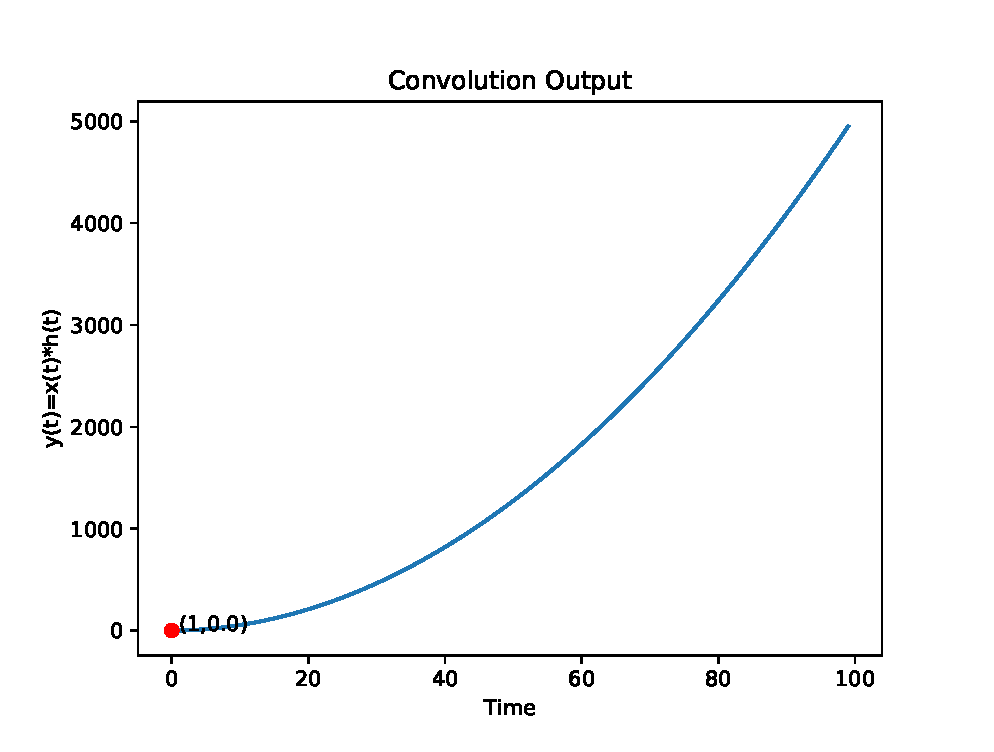
\includegraphics[width=\columnwidth]{./figs/ee18btech11048.eps}
  \caption{}
  \label{fig:ee18btech11048}
\end{figure}


The following code verifies the answer by performing convolution of the input and h\brak{t} to obtain y\brak{t} and plots the result .
\begin{lstlisting}
codes/ee18btech11048.py
\end{lstlisting}

\end{enumerate}
